\newthought{Burnside P\'{o}lya Counting} is the topic of this note. Group theory is very rich in structure\footnote{It's so rich that there are often many ways to prove some properties. I will try to write this note mostly from memory and will probably use awkward detours where more efficient ways are available.}. Its use in counting combinatorial objects is a very cool application and a fine excuse to explore it.

\subsection{Motivating Example}

\begin{marginfigure}[0.5in]
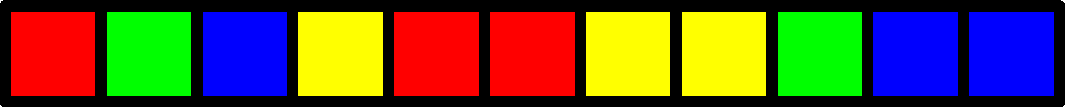
\includegraphics[scale=0.3]{single_paper_strip.pdf}
\caption{Paper strip with eleven cells colored with four colors.}
\label{fig:single_paper_strip}
\end{marginfigure}

Suppose you want to count in how many ways you can color a paper strip (like in figure \ref{fig:single_paper_strip}) with $k$ cells using $n$ colors. That is pretty simple: each cell can be colored in $n$ ways independent of any other cell and there are $k$ cells, so there are $n^k$ ways to color the strip of paper. Now let us throw in a wrinkle: from a counting perspective a strip rotated by $180$\textdegree\ is considered the same as the original strip, so the two strips seen in figure \ref{fig:paper_strips} should be counted as one strip.

\begin{marginfigure}[0.5in]
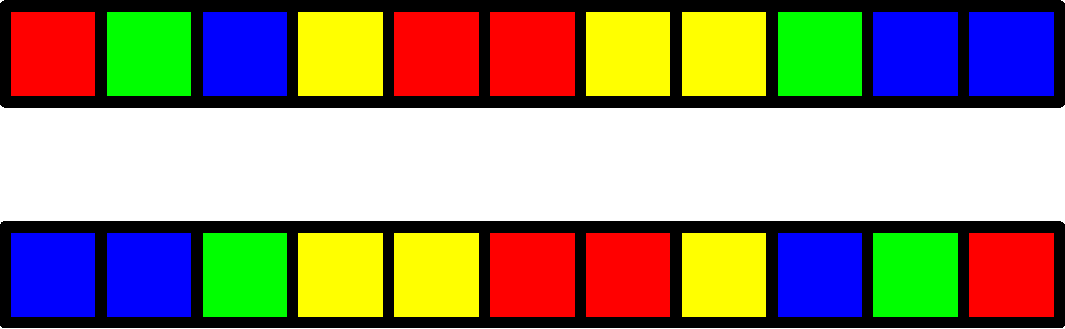
\includegraphics[scale=0.3]{paper_strips.pdf}
\caption{These two strips are the same and contribute one to the counting. The bottom strip has the reversed color sequence of the top strip.}
\label{fig:paper_strips}
\end{marginfigure}

You would say that's fine. We just divide by two and get $\frac{n^k}{2}$. Each color sequence and its inverse are considered one strip. That is almost right. There exist color sequence palindromes like the one in figure \ref{fig:paper_strip_palindromes}. In those cases rotating the strip does not result in a new color sequence, so it is not correct to divide those by two  since there is only one color sequence associated with a strip. We would be undercounting.

\begin{marginfigure}[0.5in]
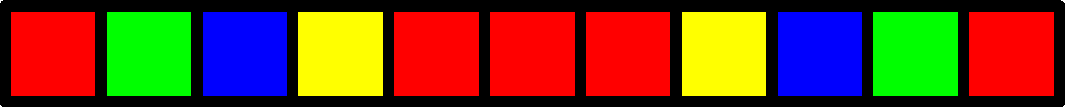
\includegraphics[scale=0.3]{paper_strip_palindromes.pdf}
\caption{Strip with a color sequence that is the same when read backwards.}
\label{fig:paper_strip_palindromes}
\end{marginfigure}

So you say fine: we first put those to the side and then divide the rest by two. Our counting total becomes counting color sequences that are not palindromes and dividing that number by two and counting all color sequences that are palindromes. Let's do that. Let $S$ be the set of colored paper strips with color sequences that are not palindromes and let $P$ be the set of colored paper strips with color sequences that are palindromes. 

There are $n^k$ color sequences and $|P|$ of them are palindromes. So

$$
\text{number of ways to color a strip} = |S| + |P| = \frac{n^k - |P|}{2} + |P| = \frac{n^k}{2} + \frac{|P|}{2}
$$

We need to determine the number of palindromes. The color choice of the first cell also determines the color of the last cell (because it needs to be the same when read backwards). Similarly the color choice of the second cell determines the color of the next to last cell and so on. So we only have half the choices of an unconstrained color sequence. Therefore

$$
|P| = 
\begin{cases}
n^{\frac{k}{2}}, \text{ when } k \text{ is even}\\
n \times n^{\frac{k-1}{2}} = n^{\frac{k+1}{2}} , \text{ when } k \text{ is odd}
\end{cases}
$$

By using the ceiling function we can collapse the two cases into: 

$$
|P| = n^{\lceil \frac{k}{2} \rceil}
$$

and get

$$
\text{number of ways to color a strip} = \frac{n^k}{2} + \frac{n^{\lceil \frac{k}{2} \rceil}}{2}
$$

This wasn't too bad but one could imagine that more complicated counting scenarios with objects where different configurations are considered the same can become quite tricky without a systematic approach\footnote{For example colored necklaces where rotation and flipping is considered the same object. Or counting how many different molecules you can form with a given number of carbon, hydrogen and bromine atoms.}. Let's look back at the colored paper strips. Maybe we can tickle out a systematic approach.

We reasoned with colored sequences. A colored sequence and its flipped counterpart were assigned to a strip. Let's look closer at the flipping. Flipping a sequence is an action on the sequence. How do these actions combine? Flipping it again brings it back to the original sequence, so flipping it twice is like doing nothing. Seems like we also need something that represents doing nothing. This points to the additive group $\mathbb{Z}_2$ with zero being the action of doing nothing and one the action of flipping. But what is an action? From what we just described, an action binds an element of the group $\mathbb{Z}_2$ with an element of the set of colored sequences (let's name this set $C$) and returns a new element of $C$. It is a function:

$$
\Phi: \mathbb{Z}_2 \times C \mapsto C
$$

To be consistent with group structure we want to impose restrictions on the function $\Phi$ and require that it satisfy two properties: 

Firstly, the action of the neutral element of the group (in our case it is zero) should not change the color sequence: 

$$
\forall c \in C: \Phi(0, c) = c
$$

And secondly, a sequence of actions should be consistent with the group operation:

$$
\forall c \in C \text{ and } \forall g, h \in \mathbb{Z}_2: \Phi(g + h, c) = \Phi(g, \Phi(h, c))
$$

With our simple group of only two elements we get $\forall c \in C$:

\begin{align*}
\Phi(0, c) &= c \\
\Phi(1, c) &= \bar{c} \text{ where } \bar{c} \text{ is the reversed color sequence of } c
\end{align*}

The number of ways to color a strip is a sum of two expressions:

$$
\text{number of ways to color a strip} = \frac{n^k}{2} + \frac{|P|}{2}
$$

The numerator in the first expression is $n^k$, the size of $C$, which is also the size of the subset of elements left unchanged by the action of the neutral group element zero (since that is the full set $C$ according to our first restriction on $\Phi$). The numerator in the second expression is $|P|$, the size of the subset of elements left unchanged by the action of the group element one (the flipping). This coincides with the set of color sequences that are palindromes. The denominator in both cases is two, the size of the group.

We are going to make a \textbf{bold statement} and posit that this counting holds for any group and any set: the number of object classes is the sum of the sizes of subsets that are invariant to the action of a group element, with the sum taken over all group elements and then divided by the size of the group.

But first we have to be more precise in describing what we mean by the general case and what we mean by object classes.

\subsection{Defining Group Action, Orbit and Stabilizer}

Given is a finite set $X$ and a finite group $(G, \circ)$ with neutral element $e \in G$ and $g^{-1}$ the inverse of $g$. 

\begin{defn}\label{groupaction}
Group $(G, \circ)$ acts on set $X$ through a function $\Phi: G \times X \mapsto X$ iff $\Phi$ satisfies

\begin{align*}
&\forall x \in X: \Phi(e, x) = x \\
&\forall x \in X, \forall g, h \in G: \Phi(g \circ h, x) = \Phi(g, \Phi(h, x))
\end{align*}
\end{defn}

The group action immediately implies some interesting subsets of $X$ and $G$. Lets define them:

\begin{defn}\label{orbit}
The \textbf{orbit} of $x \in X$ is a subset $O_x \subset X$ of all the group actions from $G$ on $x$:

$$
O_x = \{\Phi(g, x): g \in G\}
$$
\end{defn}

Orbits are precisely the object classes we mentioned above that we want to count. In the motivating example above, the orbits are the color strips and the set $X$ is $C$, the set of color sequences. So our goal is to count the number of orbits.

\begin{defn}\label{stabilizer}
The \textbf{stabilizer} of $x \in X$ is a subset $S_x \subset G$ of all the group elements of $G$ that keep $x$ unchanged:

$$
S_x = \{g \in G: \Phi(g, x) = x\}
$$
\end{defn}

In the motivating example above, for a given color sequence, the stabilizer is either the whole group $\mathbb{Z}_2$ if the sequence is a palindrome, or the stabilizer is the one element set containing just zero if the color sequence is not a palindrome.

\begin{thm}\label{orbitspartition}
The orbits of a group action partition the set $X$.
\end{thm}

\begin{proof}
We will show that group action induces an equivalence relationship $\sim$ on $X$.
We define 
$$
\forall x, y \in X: x \sim y \text{ iff } y \in O_x
$$
and show that it is an equivalence relationship. Since $\Phi(e, x) = x$ we have $x \in O_x$, so $\sim$ is reflexive.

Now assume $x \sim y$, which implies $y \in O_x$, so there is a $g \in G$ such that $y = \Phi(g, x)$. Then

\begin{align*}
\Phi(g^{-1}, y) &= \Phi(g^{-1}, \Phi(g, x)) \\
                &= \Phi(g^{-1} \circ g, x) \\
                &= \Phi(e, x) \\
                &= x
\end{align*}

so $x \in O_y$ and $y \sim x$, ie the relationship is symmetric.

For transitivity, assume $x \sim y$ and $y \sim z$, so there are $g,h \in G$ such that $y = \Phi(g, x)$ and $z = \Phi(h, y)$. We have

\begin{align*}
z &= \Phi(h, y) \\
  &= \Phi(h, \Phi(g, x)) \\
  &= \Phi(h \circ g, x)
\end{align*}

so $z \in O_x$ and $x \sim z$.

\end{proof}


\begin{thm}\label{stabilizersubgroup}
The stabilizer $S_x$ of $x \in X$ is a subgroup of $G$.
\end{thm}

\begin{proof}
For all $g, h \in S_x$ we have:

$$
\Phi(g \circ h^{-1}, x) = \Phi(g, \Phi(h^{-1}, x))
$$

but 

\begin{align*}
\Phi(h^{-1}, x) &= \Phi(h^{-1}, \Phi(h, x)) \text{ because } h \in S_x\\
                &= \Phi(h^{-1} \circ h, x) \\
                &= \Phi(e, x) \\
                &= x
\end{align*}

so 

$$
\Phi(g \circ h^{-1}, x) = \Phi(g, \Phi(h^{-1}, x)) = \Phi(g, x) = x
$$

because $g$ is also in $S_x$. It follows that $g\circ h^{-1} \in S_x$.

\end{proof}

To recap the two important properties: the orbits partition $X$ and a stabilizer is a subgroup of $G$.

We are now going to make a slight detour into the world of left cosets.

\subsection{Left cosets}

Given is a group $G$ and a subgroup $U$ (for notational simplicity in this subsection we will use multiplicative notation for the group operation and say $1_G$ is the neutral element). We define the following relationship\footnote{Note that even though we use the same $\sim$ symbol in this subsection, it is a different relationship from the relationship in $X$ in the previous subsection.} in $G$:

$$
\forall g, h \in G: g \sim h \text{ iff } g^{-1}h \in U
$$

We will show that this relationship is an equivalence relationship. For reflexivity, it's clear that $g^{-1} g = 1_G \in U$, so $g \sim g$. For symmetry we have $g \sim h$, so $g^{-1}h \in U$. But the inverse of an element from the subgroup is also in the subgroup, so $(g^{-1}h)^{-1} = h^{-1}g \in U$, therefore $h \sim g$. For transitivity assume $g \sim h$ and $h \sim f$, then $g^{-1} f = (g^{-1} h) (h^{-1} f)$. Both $g^{-1} h$ and $h^{-1} f$ are in $U$ according to our assumption, so their composition is too. Therefore $g \sim f$.

Lets denote the set of equivalence classes from this relationship with $\sfrac{G}{U}$. Let $gU = \{gu: u \in U\}$.

For every $g \in G$ let $[g]$ be the equivalence class for which $g$ is a representative. We prove that $gU = [g]$: 

Let $h \in gU$. Then there exists an $u \in U$ such that $h = gu$, so $g^{-1}h = u$ and $g \sim h$ according to the definition of $\sim$. This means that $gU \subseteq [g]$.
Likewise let $h \in [g]$. Then $g \sim h$ and $g^{-1} h = u$ for some $u \in U$. This means that $h = gu$ and $h \in gU$, so $[g] \subseteq gU$.

For every $g \in G$ the function $f_g : U \mapsto gU$ with $f(u) = gu$ is a bijection\footnote{Easy to see using the group axioms.}. This means that all equivalence classes have the same size, namely $|U|$ and we have:

$$
|G| = |U| |\sfrac{G}{U}|
$$

This concludes our small detour\footnote{There is a lot more to explore about cosets. I did say that group theory is rich in structure. We only pulled in what was absolutely needed to continue.}. Let's go back to the group actions and use what we just established.

\subsection{Burnside's Lemma}

We already know that a stabilizer is a subgroup of $G$. We can now use

$$
|G| = |S_x| |\sfrac{G}{S_x}|
$$

But what are the elements of $\sfrac{G}{S_x}$ ? We know from the detour subsection that the equivalence classes have the form $gS_x$ for some $g \in G$. Now assume $g \notin S_x$. That means $\Phi(g, x) = y$ for some $y \neq x$ in $X$. But that $y$ belongs in the orbit of $x$. There are $|O_x|$ such distinct $y$ and therefore $|O_x|$ equivalence classes. We have just proved the \textbf{orbit-stabilizer theorem}:

\begin{thm}\label{orbitstabilizer}
For every $x \in X$ we have $|G| = |S_x| |O_x|$.
\end{thm}

\begin{marginfigure}[0.5in]
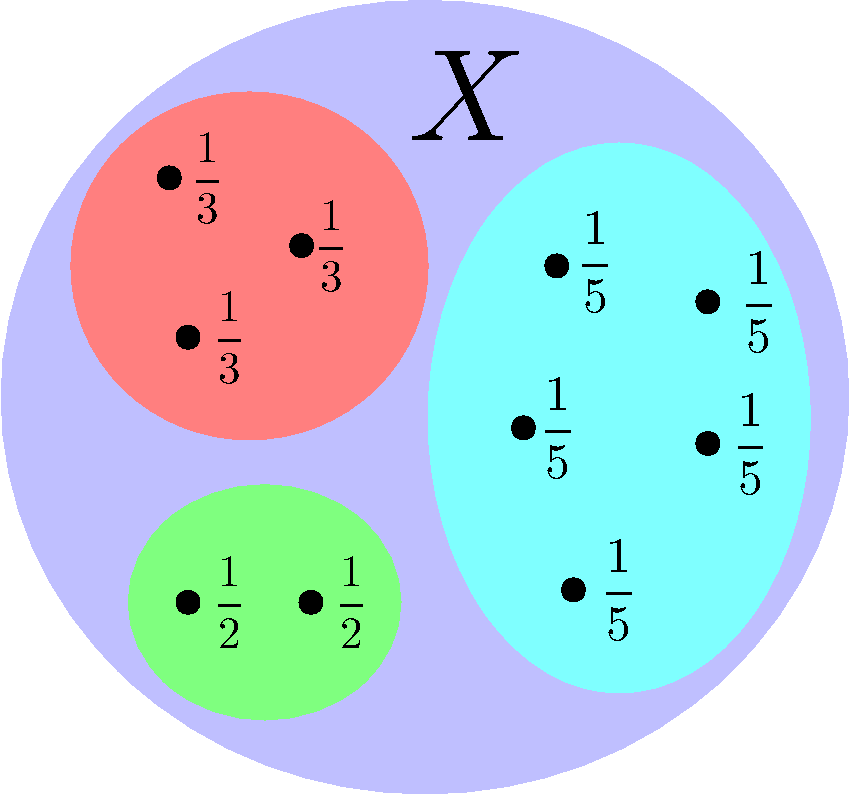
\includegraphics[scale=0.3]{orbitpartitions.pdf}
\caption{The set $X$ with three orbits. Each element in an orbit is assigned the fraction one over the size of the orbit.}
\label{fig:orbitpartitions}
\end{marginfigure}

With the help of this theorem we can count the number of orbits. We remember that the orbits partition $X$. In each orbit $O_x$ we can assign $\frac{1}{|O_x|}$ to each member of the orbit. Summing up these assigned fractions results in the value one for each orbit. So summing up the fractions over all the elements of $X$ counts the number of orbits as seen in figure \ref{fig:orbitpartitions}. The number of orbits becomes:

$$
\#orbits = \sum_{x \in X} \frac{1}{|O_x|}
$$

From the orbit-stabilizer theorem we know that $\frac{1}{|O_x|} = \frac{|S_x|}{|G|}$, so:

$$
\#orbits = \frac{1}{|G|} \sum_{x \in X} |S_x|
$$

This is already pretty good but has the disadvantage that we sum over the elements of $X$, which can be large. We want to instead sum over the elements of $G$. Let's look at the definition of $S_x$ again: 

$$
S_x = \{g \in G: \Phi(g, x) = x\}
$$

Evaluating the size of $S_x$ is equivalent to counting all pairs $(g,x) \in G \times X$ where $\Phi(g, x) = x$ for one particular $x$ and all $g$. Summing up all these sizes is equivalent to doing it for all $x$ and all $g$. We can use an indicator function to express this: $1_\Phi: G \times X \mapsto \{0,1\}$ with

$$
1_\Phi(g, x) = 
\begin{cases}
1, \text{ when } \Phi(g, x) = x\\
0, \text{ when } \Phi(g, x) \neq x
\end{cases}
$$

Then $|S_x| = \sum_{g \in G} 1_\Phi (g, x)$ and 

$$
\#orbits = \frac{1}{|G|} \sum_{x \in X} \sum_{g \in G} 1_\Phi (g, x)
$$

We can now invert the double sum order and write

$$
\#orbits = \frac{1}{|G|} \sum_{g \in G} \sum_{x \in X} 1_\Phi (g, x)
$$

Collecting all the indicator values for one fixed $g$ is the same as evaluating the size of a subset of $X$ of elements that $g$ keeps unchanged. Lets denote sets like this \textbf{fixsets}:

$$
Fix(g) = \{x \in X:  \Phi(g, x) = x\}
$$

so $|Fix(g)| = \sum_{x \in X} 1_\Phi (g, x)$.

Using this we arrive at our first milestone, the \textbf{Burnside Lemma}:

$$
\#orbits = \frac{1}{|G|} \sum_{g \in G} |Fix(g)|
$$

\subsection{Applications of the Burnside Lemma}

As a first application of our lemma, lets revisit the motivating example of color strips and verify that we get the same answer. According to the lemma we have

$$
\text{number of ways to color a strip} = \frac{1}{|\mathbb{Z}_2|} (|Fix(0)| + |Fix(1)|)
$$

Clearly $Fix(0)$ are all the color sequences, so $|Fix(0)| = n^k$ and $Fix(1)$ are the color sequences left unchanged by flipping, ie palindromes, so $|Fix(1)| = n^{\lceil \frac{k}{2} \rceil}$. Our answer checks out.

\begin{marginfigure}[0.5in]
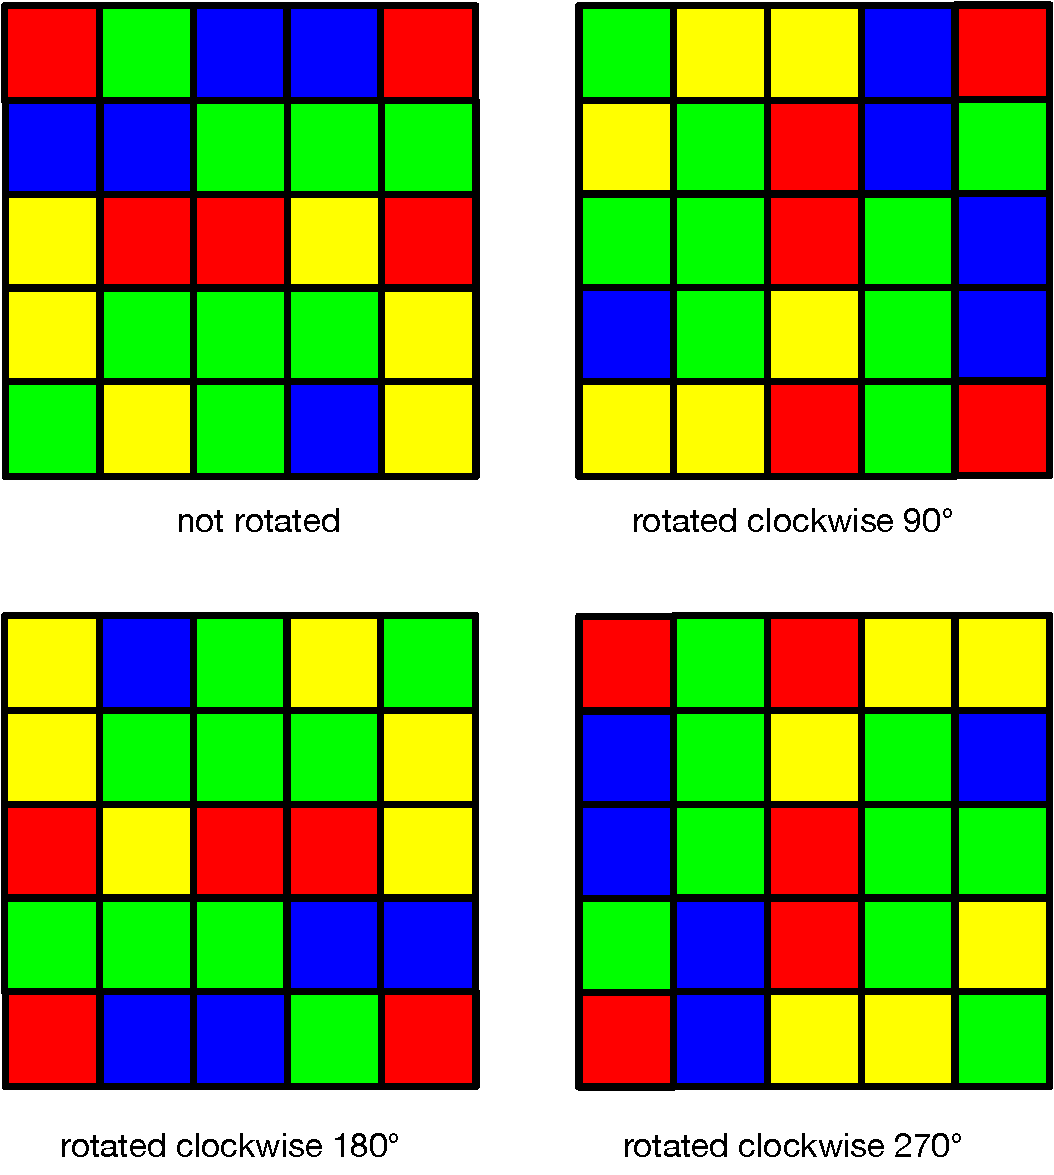
\includegraphics[scale=0.3]{tableclothorbit}
\caption{These four configurations are considered to be the same tablecloth.}
\label{fig:tableclothorbit}
\end{marginfigure}


The second example is a square tablecloth of five by five cells to be colored with four colors. Here rotations by $90$\textdegree, $180$\textdegree\ and $270$\textdegree\ are considered the same tablecloth as seen in figure \ref{fig:tableclothorbit}. This is very similar to our first example, but here the group acting on the set of color sequences is the cyclic group $\mathbb{Z}_4$. In how many ways can we color the tablecloth? To apply Burnside we need the sizes of four fixsets. We again have $|Fix(0)| = 4^{25}$, ie all color sequences are unchanged by not rotating. 

$Fix(1)$ is the set of color sequences unchanged by rotating by $90$\textdegree. If we divide the cloth into four quadrants (assigning shared boundary cells like in figure \ref{fig:tableclothquadrants}), it's clear that a $90$\textdegree rotation forces the contents of each quadrant to move to the next quadrant. So if the color sequence is supposed to stay unchanged then all four quadrants must have the same contents. The exception is the cell in the middle of the tablecloth. It is unchanged by any rotation. Therefore $|Fix(1)| = 4 \times 4^{6}$.

\begin{marginfigure}[0.5in]
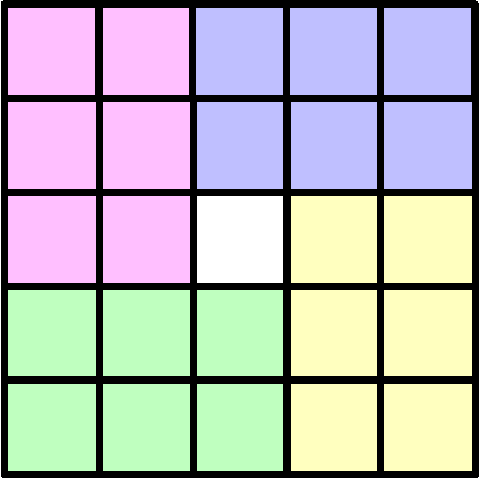
\includegraphics[scale=0.4]{tableclothquadrants}
\caption{The four quadrants of the tablecloth.}
\label{fig:tableclothquadrants}
\end{marginfigure}

$Fix(2)$ is the set of color sequences unchanged by rotating by $180$\textdegree. The quadrants across from each other end up exchanging contents which means those contents have to be equal for the color sequence to by unchanged by the rotation. Therefore $|Fix(2)| = 4 \times 4^{12}$.

And finally $Fix(3)$ is the set of color sequences unchanged by rotating by $270$\textdegree. The quadrants exchange contents with the quadrant before them (in clockwise order). Therefore $|Fix(3)| = 4 \times 4^{6}$.

\begin{align*}
\text{number of ways to color tablecloth} &= \frac{1}{4} (4 \times 4^{6} + 4 \times 4^{12} + 4 \times 4^{6}) \\
                                          &= 2 \times 4^{6} + 4^{12} \\
                                          &= 16785408
\end{align*}


